\chapter{Experimental setup} 
\begin{itemize}
\item description of MAMI, how the beam is produced, how the electrons are polarized.
\item description of A1.
\item description of beam stabilization, how the monitors measure the beam parameters.
\item Electronics description, DAQ system, VFC monitors.
\item Detectors A and B.
\end{itemize}

\section{First description of the experiment} \label{FirstDescription}

{\bfseries First description of the experiment, how we want to collect data, new picture of the kinematic of the experiment. Maybe here it's a good point to describe the structure of the event}
To measure the Beam-Normal single spin asymmetry, a polarized beam of $ \SI{570}{\mega \electronvolt}$ will be sent against a $\SI{10}{\milli \meter}$ $^{12}C$ target. The detectors consist of two fused-silica coupled to 3 (detector B) and 8 (detector A) pmts, which collect the Cherenkov light emitted when an electron pass through the fused-silica. 
The detector are placed inside the two spectrometer of the A1 hall, which are not used in this experiment due to the high luminosity of the beam ($ \SI{20}{\micro \ampere}$) that is away from their good point of operation. 
The photomultipliers asymmetry due the change of the electrons spin is the target of the measurement. The pmts signals are collected and digitalized by the \textbf{NINO} board, after a threshold selection, and sent to the A1 control room computer, where the DAQ program collect the data together with all the data coming from the Beam monitors producing Binary files, which are later analyzed by the analysis program, which is significant part of the work done in the framework of the thesis. 
The data collected are divided in \textit{Events} made by 4 \textit{sub-events} in sequence. Each event correspond to a temporal window of $\simeq \SI{80}{\micro \second}$, where each sub-event is $\SI{20}{\micro \second}$ long. Here it's important to clarify that unlike the majority of experiments in high energy physics, an event is made by all the electrons interacting with the detectors during the time interval of the event, and we will refer to this hereafter unless otherwise stated. The division into sub-events reflects the polarization sequence of the beam. The PMTS counts and the beam monitor values are saved for each subevent, along with the time lenght of the event measured by in clock cycle by the NINO electronic board which is descrribed in \ref and other values which are required to process beam monitor data.\\ 

The general structure of the event is the following: 

\begin{figure}[hbtp]
\centering
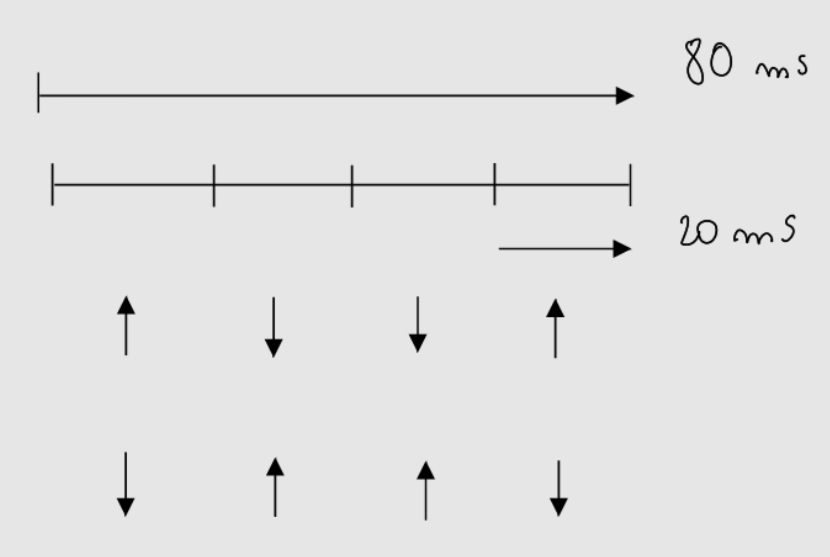
\includegraphics[width = 0.45\textwidth]{figures/EventStructure.jpg}
\caption{Event structure}
\end{figure}

\newpage
\section{Mami}
How Mami produces polarized electron and how the particle are accelerated (the way Mainz Mikroton is working is completely different from the other accelerators, so maybe this section will be too long).

\subsection{Acceleration stage}
explain how electrons are accelerated, and sent to different experiments.

\subsection{Polarized Beam}
{\bfseries Here a subsection to explain how the polarized electrons are produced. Important to mention the systematic error for the polarization mesurement (in our beam time we couldn't measure with Moller polarimeter, so this discussion is important for future experiment, however it's important to say something about it). Remember to explain how the spin are rotated to the transverse plane, and the $\frac{\lambda}{2}$}

For the beam-normal single spin asymmetry a vertical polarized beam is necessary. At the MAMI electron accelerator is possible to produce a vertical polarized beam with energy in the range $\SI{180}{\mega \electronvolt} - \SI{855}{\mega \electronvolt}$ \cite{Schlimme_2017}. In this section the procedure to orient the beam vertically is presented, following an explanation of how the degree of polarizarion of the beam is measured. \medskip

The electron source used at MAMI is made by a strained GaAs/GaAsP superlattice photocathode illuminated by circular polarized light. A Pockels cell changes the helicity of the photons impinging on the electrons. The extracted electron has the same helicity of the incoming photon, let's suppose as an example:

\begin{center}
\begin{equation}
\feynmandiagram [scale = 0.8, transform shape][baseline = (g)]{
	a [particle = \(e^{-}\)] -- [fermion] b  -- [fermion] c [particle = \(e^{-}\)],
	b -- [boson] d [particle = \(\gamma\)],};
\hspace{2cm}
(Jz)_{\gamma} = \pm 1 \qquad (Jz)_{e^{-}} = \mp \frac{1}{2} \rightarrow \pm \frac{1}{2}
\end{equation}
\end{center}

With the fast change of the Pockels cell it is possible to alternately revert the sign of the polaritazion. By the insertion of a $\lambda/2$ plate between the laser system and the photochatode the polarization orientation of the electron beam can be reversed for each sub-event, useful later for the estimation of systematic errors. The beam polarization achieved with this source is roughly $80 \% $, for the beam time it was : $0.79 \% $

To switch from longitudinal polarization to transverse polarisation, two devices are used: the \textbf{Wien filter} and a \textbf{double solenoid} located in the injection beam line. 

\begin{figure}[hbtp]
\centering
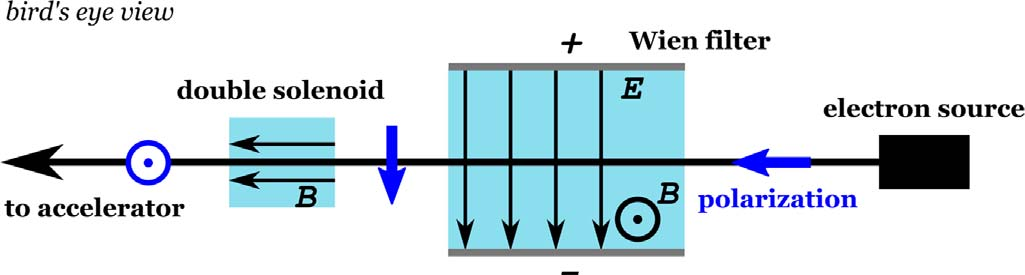
\includegraphics[width = \textwidth]{ExperimentalSetup/injection.png}
\caption{Setup for the trasverse polarization.}
\end{figure}

Following the picture, the longitudinal polarized electron from the source are rotated first in the XY plane, to obtain the trasverse polarization, then with subsequent double solenoid the spins are rotate in the vertival direction. 
After this allignement the electrons go through the accelerator to the experimental hall. The spins then precesses during this time in the magnetic fields of the accelerator's bending magnets, following the BMT equation.
In our experiment, because of the vertical polarization, only the residual horizontal component precedes during the motion. For conventional experiment the polarization vector is rotated by the Wien filter with an angle such that the polarization si longitudinally aligned in the experimental hall, considering that after the rotation, the polarization is affected by another rotation due to the spin precession. The rotation angles of the polarization vector through the accelerator are known from simulations and are also directly measured for relevant energies, for a beam of $\SI{570}{\mega \electronvolt}$ the rotation angle is $\ang{55}$ with an accuracy of $\pm \ang{2}$
At the beginning MAMI was not developed with the aim a trasverse beam. So it's not possible to measure directly the polarization for the vertical axis. However it's possible, with the existing setup, to exstimate the degree of polarization. For this purpose a Moller, Comport and Mott polarimeters are used. The vertical polarization alignment can be accomplished by the minimization of the horizontal components. 


\subsection{Mott, Compton and Moller polarimenters}
{\bfseries Briefly explain how the Mott polarimeter works, for measuring the polarization of the beam.}

To Measure the polarization of an electron beam different polarimeters can be used. Here we explain briefly the physics underlying the \textit{Mott} polarimeter, used in the experiment.
Consider an electron beam that is sent towards a nucleus of charge $Ze$. We know from theory that the spin of the incident electron is affected by the electromagnetic field produced by the nucleus. This can be described as:

\begin{align*}
\vec{B}_{nucleus} = \frac{-1}{c} \vec{v} \times \vec{E}_{nucleus} = \frac{Ze}{mc r^{3}} \vec{L} \\
V = - \mu \cdot B_{nucleus} = \frac{Ze}{mcr^{3}} \vec{L} \cdot \vec{S}_{e^{-}}
\end{align*}

We can recognize the spin-orbit interaction here. This term yields the polarization dependence of the cross section. The cross section can be model in the following way

\begin{align*}
\sigma(\theta) = I(\theta) [1 + S(\theta) \vec{P} \cdot \vec{n} ]
\end{align*}

Here a scheme to identify the scattering process: 

\begin{figure}[hbtp]
\centering
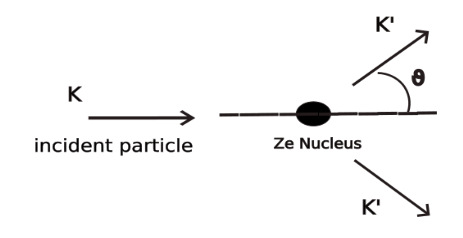
\includegraphics[width = 0.45\textwidth]{ExperimentalSetup/mottFig.png}
\caption{Scheme of the Mott scattering, the polarization is ortogonal to the plane,  $ \vec{n} = \frac{\vec{k} \times \vec{k'}}{|\vec{k} \times \vec{k'}|}$}
\end{figure}

The direction of $\vec{n}$ dependso on whether scattering to the left or right is being considered. Let's suppose our initial beam has a polarization $P$, and so we compute the asymmetry $A(\theta)$ of the scattered electrons between left ($N_{L}$) and right ($N_{R}$). $N_{L}$ and right $N_{R}$ will be proportional respectively:


\begin{align*}
N_{L} &= N_{\downarrow}[1 + S(\theta)] + N_{\uparrow}[1 - S(\theta)] \\
N_{R} &= N_{\uparrow}[1 + S(\theta)] + N_{\downarrow}[1 - S(\theta)]  \\
A(\theta) &= \frac{N_{L} - N_{R}}{N_{L} + N_{R}} = \dfrac{N_{\downarrow}(1 + S(\theta)) + N_{\uparrow}(1 - S(\theta)) - N_{\uparrow}(1 + S(\theta)) + N_{\downarrow}(1 - S(\theta))}{N_{L} + N_{R}} = ... = P \cdot S(\theta)
\end{align*}

From the last equation we have a relation which give the beam polarization in terms of $A(\theta)$ (which is what is measured) and the asymmetry function $S(\theta)$ (known also as Sherman function). There are several calculation of the Sherman function, which is well-known for high energy electron scattering.

The total beam polarization is measured by a Moller polarimeter, in the experimental hall, with the beam polarization oriented longitudinally in the experimental hall. The Moller polarimeter can measure the longitudinal polarization of the beam.The other two polarimeters, Compton and Mott, located behind the injector linear accelerator (ILAC), are sensitive to the longitudinal and the trasverse horizontal components of the beam (with an energy around $\SI{3.5}{\mega \electronvolt}$ at this stage). The procedure for the allignment is the following: at the beginning of the beam time the Mott polarimeter is used for different settings of the solenoidal field, with the Wien filter angle equal (nominal) to $\ang{90}$. The aim is to minimize the horizonal polarization component after the rotation performed by the double solenoid, changing the solenoidal magnetic field. Then a second optimization follows, using the Moller polarimeter for different Wien filter angles is performed. With the new Wien filter settings, another measurement is performed with the Mott polarimeter.


\section{A1 spectrometers hall}

Describing the A1 room, how the spectrometers are operating (+ figures), a picture of the target and the important parameters, like thickness. Also mention the convention to use target with$10 \%$ of the radiation lenght, to avoid double scattering.  Mention that we need the Wobbler magnet to change the hitting position of the beam to prevent the target from melting.
Then add a picture of the beam-line.

\section{Detectors and beam monitors}

\subsection{Detectors A and B}
{\bfseries Describe the two detectors we placed inside the spectrometers, the $Q^{2}$ for our mesurement. The way the counts are collected, so the expected signal for the Čerenkov detector. Explain also how we will use the old detectors of the two spektrometers to align the elastic scattering plane to our detectors.}

The scattered electrons that hit the target are detected via two fused-silica coupled with 3 PMTs and 8 PMTs. The electrons that pass through the fused-silica (refractive index $1.45$) emits Cherenkov light that is detected by the pmts. In the old electronic setup all the current generated by the pulse signal was collected, for each time interval of a sub-event. Then the asymmety was recostructed from the integrated current. This method is affected by high noise, and can't be applied for future experiments involving lead target.
With the new electronic, all the single electron are counted, in order to work with the low rate expected from lead.


\begin{figure}[hbtp]
\centering
\subfloat[][\emph{Detector B}]
	{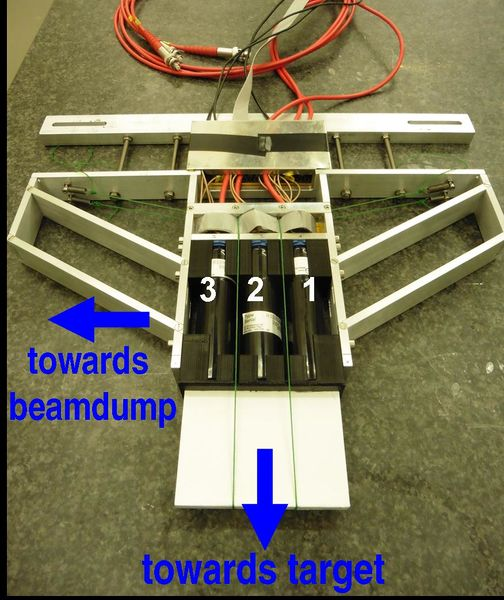
\includegraphics[width = 0.35\textwidth]{figures/504px-Blackfalcon.jpg}} \quad
\subfloat[][\emph{Detector A}]
	{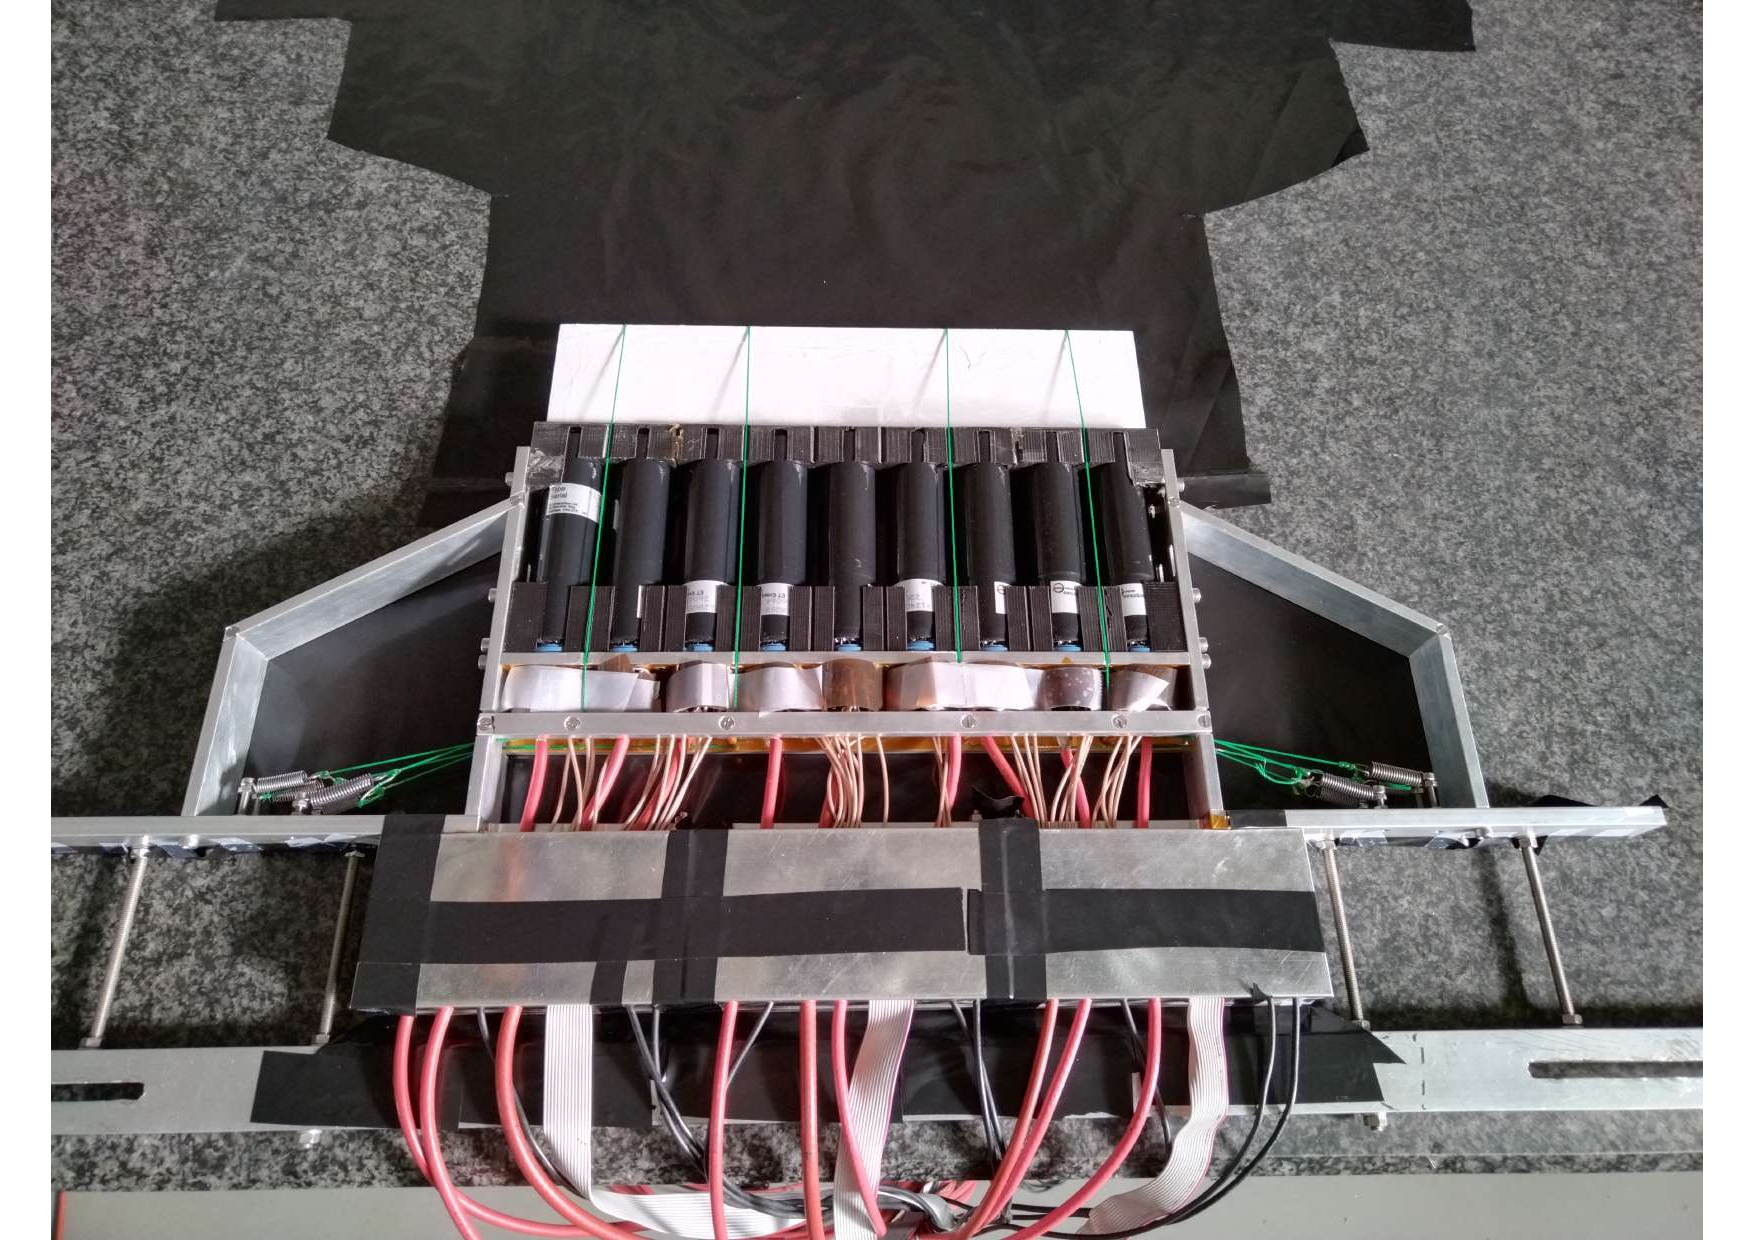
\includegraphics[width = 0.45\textwidth]{figures/IMG_20221110_122246.jpg}} \quad
	\label{fig:Detectors}
\end{figure}

The fused silica size for detector B is $(\SI{7}{\centi \meter},\SI{10}{\centi \meter})$. 

\subsection{Monitors and stabilization}
{\bfseries Explain how the monitors for the beam parameters work. (this section could be long, however the way these parameters are measured is particular, so it's important to explain everything properly).}

\section{Electronics}
{\bfseries Short introduction about the old electronics setup and why a new versions is needed, then describe all the electronics used for our experiment:}
\begin{itemize}
\item Nino board for collecting the data from the pmts
\item VFCs for collecting the data from X21,X25,Y21,Y25,ENMO,I21,I13
\item master board for collecting the monitors data/controlling the source/wobbler magnets.
\item small boxes for switching from new electronic read-out to the old electronics read-out (spectrometers DAQ)
\end{itemize}


\subsection{VFCs}

Some parameters which describe the beam are needed in order to take into account possible effect in the measure of the Trasverse asymmetry. The relevant data are the position in the $(x,y)$ plane, the incident angles on the target, the current and energy of the beam. All this values are collected using the already existing monitors. \\
To collect the data from the monitors, single and multichannel, synchronous voltage-to-frequency converters (AD7742) are used. This devices contain an analog modulator that is able to convert the input voltage into an output pulse train, whose frequency is proportional to the input voltage. 

\begin{wrapfloat}{figure}{I}{0pt}
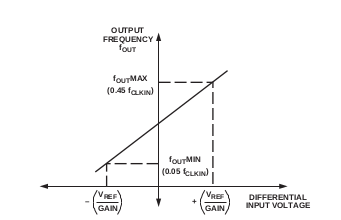
\includegraphics[width=0.5\textwidth]{ExperimentalSetup/Vfc.png}
\caption{Frequency versus Voltage}
\end{wrapfloat}

The VFCs are powerd with an external tension of $\SI{5}{\volt}$, and a differential voltage input in the range ($-V_{ref}$, $V_{ref}$) is also applied. An external clock signal, that is indicated with "CLKIN" is provived as a reference signal for the oscillator frequency.
The analog input signal is sampled with by a switched capacitor, with a rate that is controlled by clock  that can be supplied externally, in our case we used a $\SI{6}{\mega \hertz}$. A scheme of the electronic circuit is drawn here (\textit{aggiungere figura}), the output of the Comparator  is a fixed width pulse (the pulse is initiated by the edge of the clock signal) with a frequency that goes from $0.5 \% \cdot f_{CLKIN}$ to $0.45 \% \cdot f_{CLKIN}$ \cite{VfcDatasheet}, where the first correspond to $\SI{0.0}{ \volt}$ in input and the second to $V_{ref}$. Neglecting possible systematic errors, the relation the output frequency and the input voltage is the following:

\begin{equation}
V_{in} = \frac{V_{ref}}{40 \% \cdot f_{CLKIN}} (f_{out} - 5\% f_{CLKIN})
\end{equation}

We control the $f_{CLKIN}$ with the period of the clock. The data are acquired counting the number of pulses that come from the comparator, so we can substitute to $f$ the number of pulses (the two quantities are proportional), and we end with:

\begin{equation}
V_{in} =  V_{ref}[2 \cdot \dfrac{N_{pulses} - 5 \% N_{CLKN}}{40 \% N_{CLKN}} - 1]
\end{equation}

\subsection{Nino board} \label{NINO}

The NINO board is our data acquisition system for the pmt counts. It is made by $32$ analog input channels and it'is power with $\pm \SI{5}{\volt}$. Each channel has an attenuator, and the signal pass through that before going to the Comparator, which compare the signal to the threshold. The Output signal is a Low-voltage differential signaling (LVDS). Each comparator can handle eight channel and for each of them it is possible to define a global threshold. With the current settings of NINO board, it is possible to change the threshold of each channel acting on another value, the attenuation, which decreases the value of the global threshold of each single channel. All the value that can be modified are 12 bit numbers, so a setting interval of $(0. ; 4095)$.

\begin{figure}[hbtp]
 
 \centering
 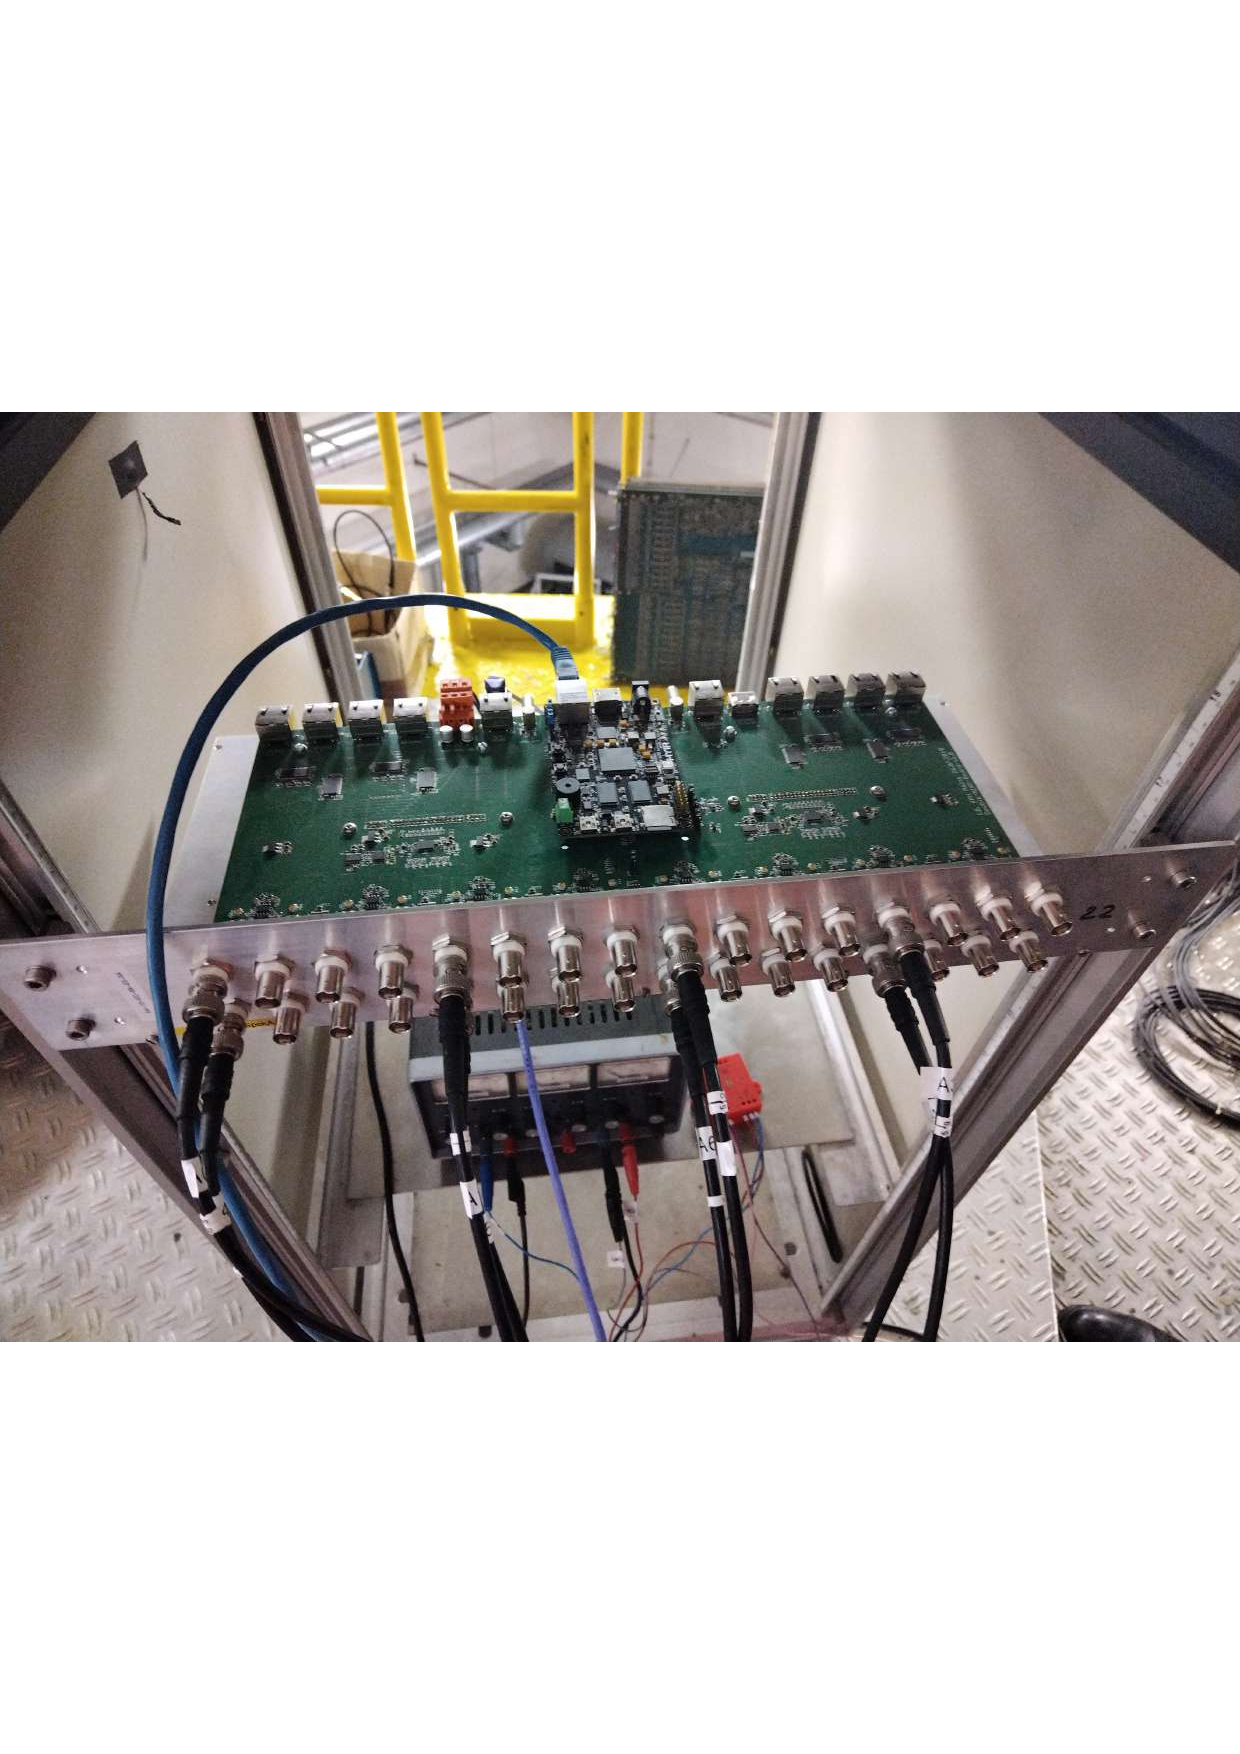
\includegraphics[scale= 0.4]{figures/NINO.pdf}
 \caption{Nino Board}
 \label{fig:NinoBoard}
 \end{figure}

Two Nino board are used in the experiment, one for detector A and one for detector B. In principle it is possible to use only 8 and 3 of the 32 channels the are ready to use, considering we have only 3 and 8 pmts to read out. However it is useful to split the analog output signal by the pmts and send it to 4 different channels. So, working with the attenuation value, we can define 4 different threshold values for each pmt. This is something that can improve the noise management. This will be implemented for the future experiments, nevertheless this was not done during our data collection.
The way we selected the threshold is explained in the following chapter (Analysis).

\subsection{Master Board}